\chapter{Hello, World!}
\newpage
\section{富士山下}
下面是获得日本早稻田大学IPS项目全奖Offer学长的申请经验。\par
\subsection{基本信息}
名字:庄系舟\par
申请:早稻田大学IPS研究生院Master\par
地点:日本九州岛 福冈县 北九州市 若松区\par
时间:9月;两年制\par
其实是考研没好好准备,考跪了……于是就试着申请了一下IPS。这个offer运气占多,早大给了150w日元/年+免学杂费,给挺多的,于是就去了。\par

\subsection{直接正题}
我知道很多我们院的同学都等着南大和早大的合作项目,但是其实这个项目从去年开始就没有了,所以还得自己申请,在这里要谢谢刘钦老师给的许多帮助,虽然是材料递交deadline的当天才通知的,不过还是很幸运,和日本方面沟通了一下,给了两天延缓期限,让我们完成申请材料。\par
申请没有什么硬性要求,完全是本着宽进严出的方针(不过Master毕业也挺容易的)
入学后先一个学期的通识基础课程教育,学分修满后再选择导师和实验室,和其他学校有所不同。\par

\subsection{申请时间}
申请的窗口期每年有两个,分别是1月和4月。早大的开学可以选择春季或者秋季,像我们大部分人应该是选择秋季的9月开学,要申请的同学请多多关注早大的官网,窗口期会提供申请材料的下载,请大家仔细阅读材料中的guide手册。

\subsection{语言要求}
语言没有硬性的要求,有G、T的分数和日语考试的分数当然最好,没有这些也可以申请IPS。

\subsection{奖学金}
下载申请材料时,请一起下载鼎新奖学金申请表,填写后一起寄出,随后等待电面,电面完半个月后出结果。
如果这个奖学金申请成功了,就没办法再申别的了。

\subsection{必要材料}
\begin{figure}[htbp]
\centering
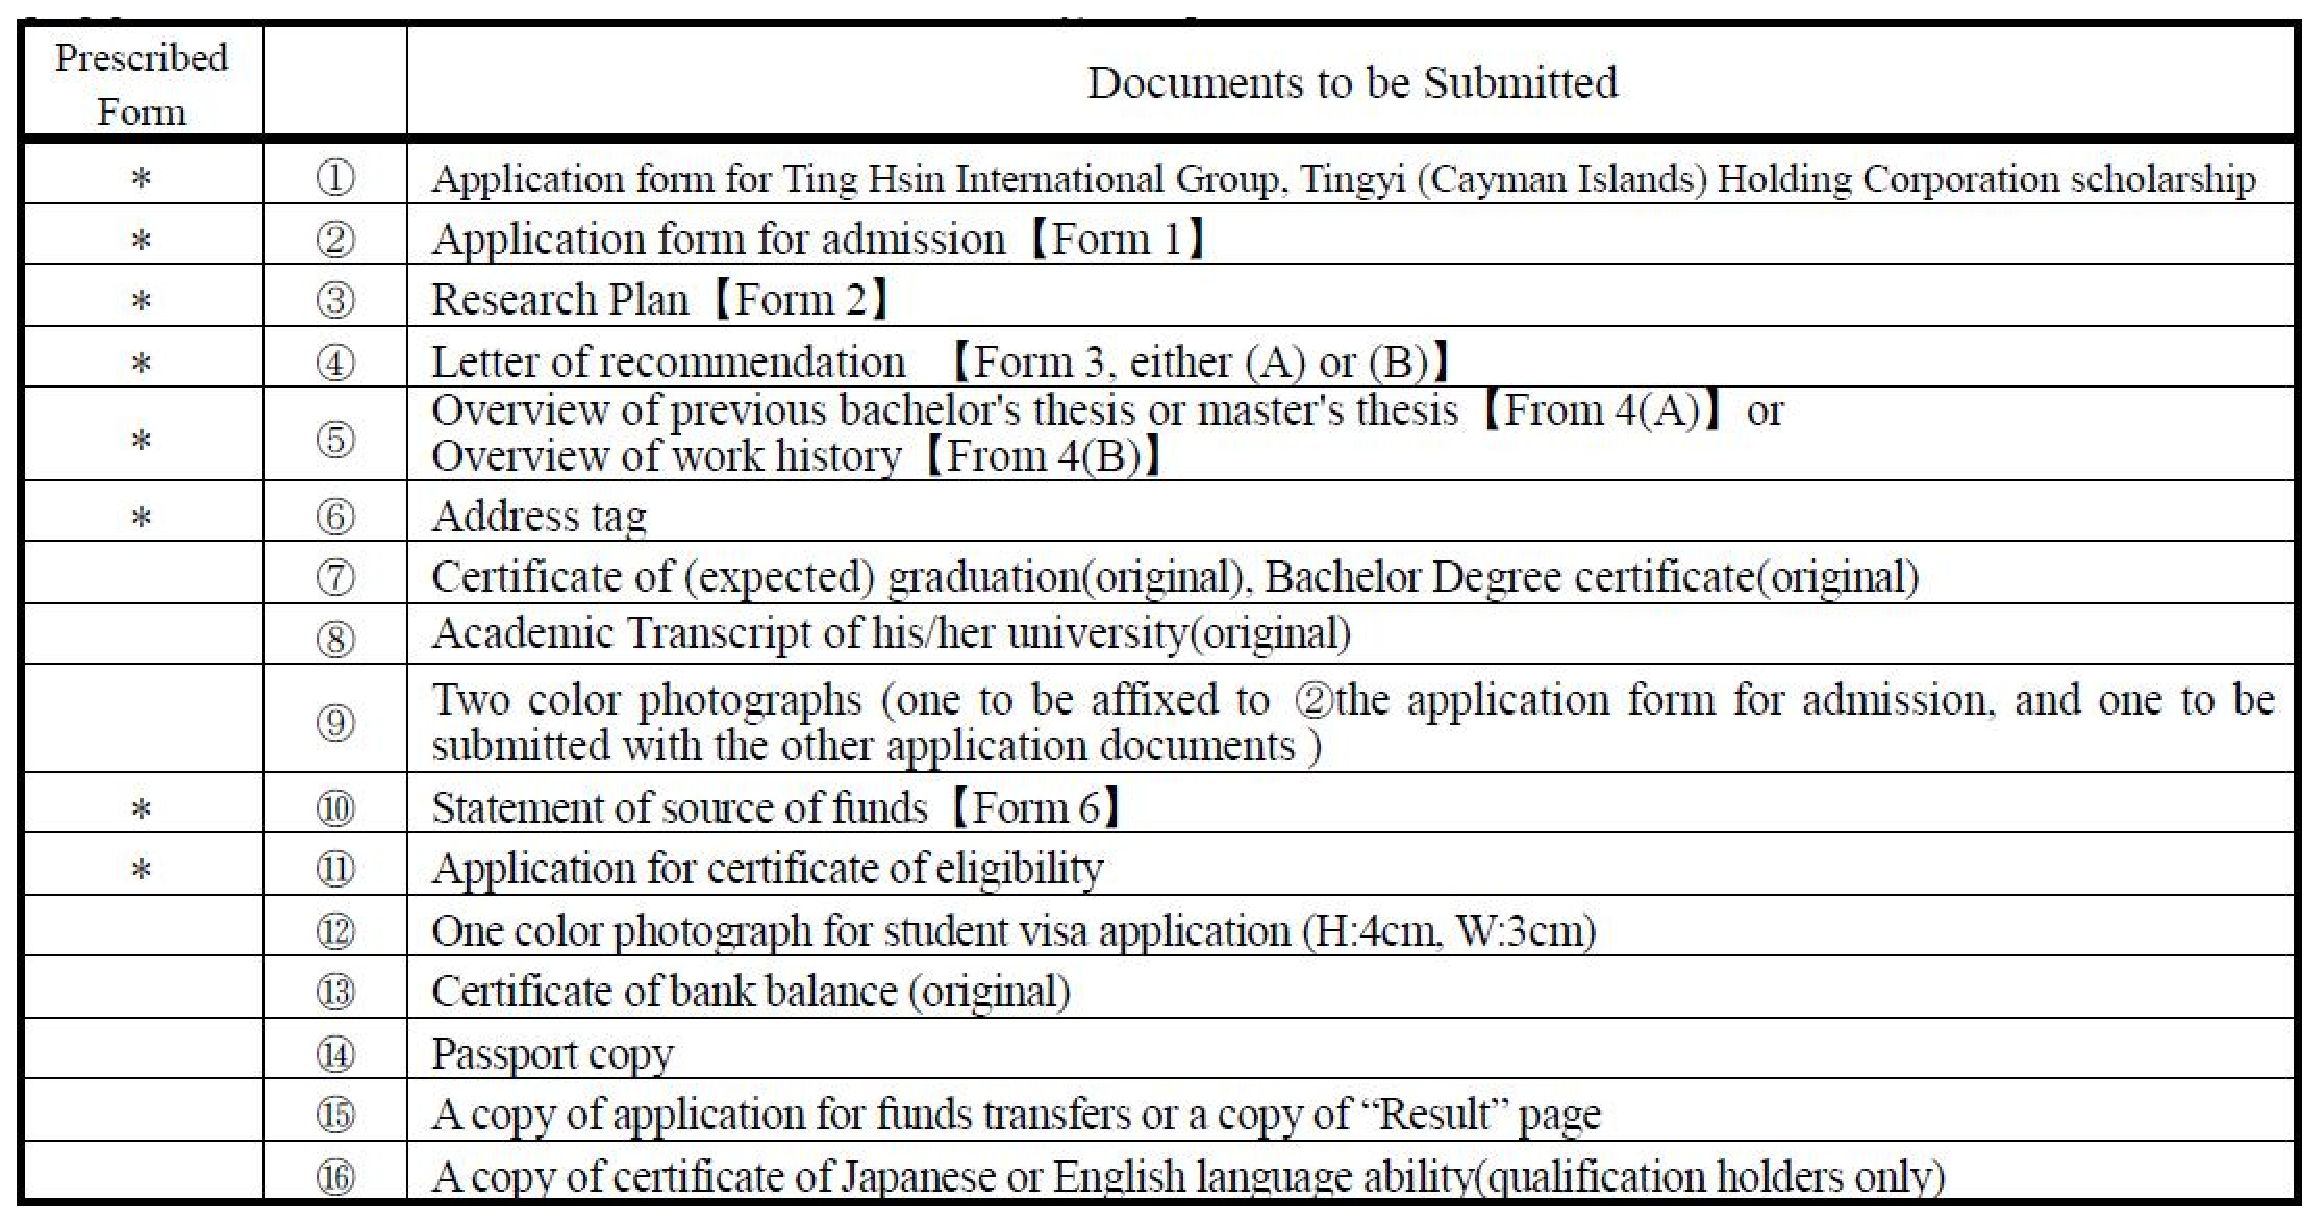
\includegraphics[width=12cm]{5allworld/cite.eps}
\end{figure}\par

其中,打*的是必须按时在deadline之前提交的,如果不申请奖学金,1可以不用提交。没打*的可以等拿到了再提交。\par
其中,1、2、3、4、5、6、10、11,也就是打*的这几项,是从网上下载表格后填写的。\par
第7项,如果还没拿到毕业证书,请到学院找辅导员和教务员开具预期毕业证明(!不是学校教务处的在读证明,请让学院的教务员盖学院的公章)\par
第14项,如果没有护照,最好要在offer寄到之前办好。\par
第15项,申请需要在网上缴纳报名费,缴纳完毕后请保存缴纳成功的网页页面,并打印。\par
注意,一切以官方网站下载的指导手册为准!

\subsection{申请流程}
首先,从官网上下载申请材料:\href{http://www.waseda.jp/ips/english/index.html}{官网地址}。打印之后按要求填写完整后寄出。然后,申请奖学金的请等待电面,电面后等待email通知。最后,耐心等待EMS送来的offer。Offer里有入学流程手册和一些表格,填好个人信息,Student Card, 各种保证书,然后寄去日本,并按照入学流程手册的流程打学费过去。毕业后扫描中英文的毕业证和学位证并email给日本,英文的证件请都去校教务处办理。机票等拿到护照后,知道了入学日期后去买,别买太早的,太早了宿舍不让住,只能自己在日本租房子或者住酒店,学校的宿舍可以在开学典礼前两天入住。

\subsection{学费和住宿}
学费:第一学期77万日元,其后每学期50万日元左右\par
生活费:每月正常花销在5~6万日元左右。(不正常的开销另当别论)\par
住宿:两人间,随机分配,有独立卫浴小厨房,请自带床上用品。费用:每月1.1万日元左右


\section{维多利亚湾}
下面是一位申请到香港科技大学CS硕士的学姐经验。

\subsection{总结}
冒出要去香港读研的念头比较晚,整个准备过程都显得有些仓促,也有很多缺陷,不过好坏都是经验,在此与大家分享。\par

组成木桶的木板长短不一,如果用木桶装水,那所装水的体积主要由最短的木板决定,如果用木桶装熟透的米饭,那么可以利用最长的木板来增大木桶所装米饭的体积。在申请过程中,需要突出自己具有的优势,弥补缺陷。我的GPA较低,80出头的成绩刚好能够满足申请香港各所大学研究生的条件,但在众多竞争者中实在没有多少竞争力。较幸运的是,一年半的科研经验提高了自己的硬件条件。在本科阶段,只要曾参与到科研项目中,即使没有发表论文,都应该在简历或者面试中作出适当介绍。例如,在CV中,可以简要陈列自己曾参与的科研项目,简要描述自己在这些项目中作出的主要贡献,将已发表的论文以标准格式列出,并用粗体突出自己的名字。在PS中,除了突出自己申请该学校、该项目的原因外,也可以委婉地描述自己的优点,向学校陈述为什么评委会应该同意你的申请。申请香港大学MPhil/PhD在申请需要写RP,建议在写RP前与自己研究的课题相关的论文,在RP中可以简要描述自己的研究经历、对具体研究课题的认识(优缺点)、提出可扩展的研究方向。\par

\subsection{申请}
香港的研究生分为MSc与MPhil,MPhil需要跟随导师做项目,申请该项目的成功与否与导师的意向有很大关系,对于没有特别优势的自己来说,套磁是一个必要步骤。在确定想要申请的学校之后,还要选择好的导师,可以通过查看导师的主页、联系导师指导过的学生等多个渠道了解导师的研究方向、个性、指导原则等情况,从而从众多教授中选择出需要套磁的对象。一般情况下,可以同时联系多个学校的多个教授,以节省时间,增大几率,但是不建议同时联系同系的不同教授。在对教授进行了解时,需要知道需要的是什么样的学生,有的教授需要的是勤奋型的学生,有的教授需要的是思维灵活的学生,可以根据具体情况突出自己的优点。如果教授已经肯定了申请者的能力,鼓励申请者申请某个项目,那么申请该项目的成功率就近半了。\par

在选择推荐人时,较幸运的是能够找到与自己想要申请的教授相识的人作为推荐人。因为对于教授来说,了解大多数申请者的途径只是通过阅读CV,PS等文书,教授也会怀疑这些文书的可信度,如果这个时候能够有熟人为自己做出推荐,会增加教授对申请者的信任,提高申请的成功几率。\par

无论是CV,PS,RP还是RL,在提交之前都需要从文书组织结构与语言语法两个方面进行重复修改。这个阶段可可以找专业培训机构,或者在国外的朋友帮忙修改。这两个方法我都尝试过,在修改文书之初,我先找了南京某培训机构的一名老师,但是修改后觉得效果欠佳。后来请了一些有申请经历的朋友帮忙,重复修改了很多次,才敢提交申请文书。个人感受,如果能够找到那些了解自己并已经熟悉国外思维模式的朋友帮忙,能够为申请者节省很多精力。当然,申请者自己也需要一遍遍地对文书组织结构进行修改,一是因为申请者应该充分熟悉自己的文书内容,二是最了解申请者经历的人是申请者自己。
